\selectlanguage{german}
\subsection{Alarm-Hardware-System}
Das Alarm-Hardware-System besteht aus einem Raspberry Pi, der als zentrale Steuereinheit fungiert. An den GPIO-Pins des Raspberry Pi sind LEDs (eine gelbe, eine grüne und eine rote), ein Piezolautsprecher (Buzzer) und ein Taster angeschlossen, um sowohl visuelle als auch akustische Alarme zu erzeugen. Dieses System wird verwendet, um das Pflegepersonal sofort auf kritische Situationen wie Stürze oder die Abwesenheit eines Patienten aus dem Bett aufmerksam zu machen. Zusätzlich sind Widerstände auf einem Steckbrett montiert, um die Signale zu steuern und zu verstärken. Der Taster dient dazu, den Buzzer stummzuschalten, wenn die rote LED leuchtet.

\begin{figure}[h]
	\centering
	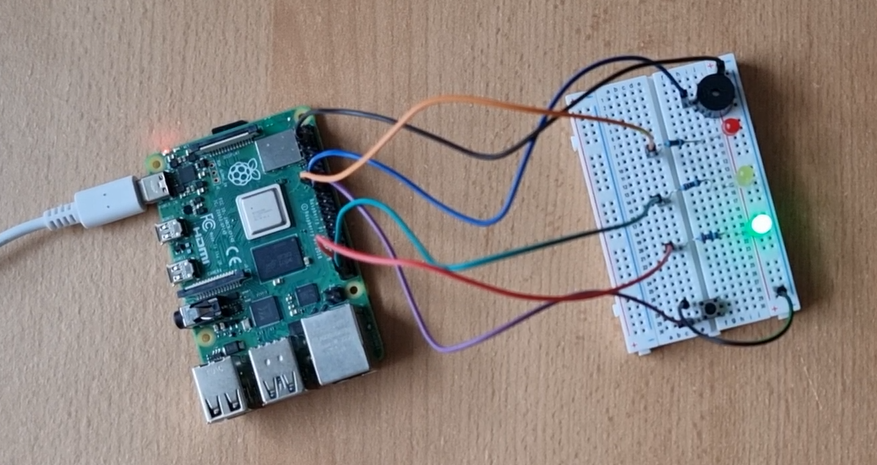
\includegraphics[width=0.8\textwidth]{images/Alarm_grun}
	\caption{Raspberry Pi mit angeschlossenem Alarm-Hardware-System (grün)}
	\label{fig:alarm_system}
\end{figure}

\begin{figure}[h]
	\centering
	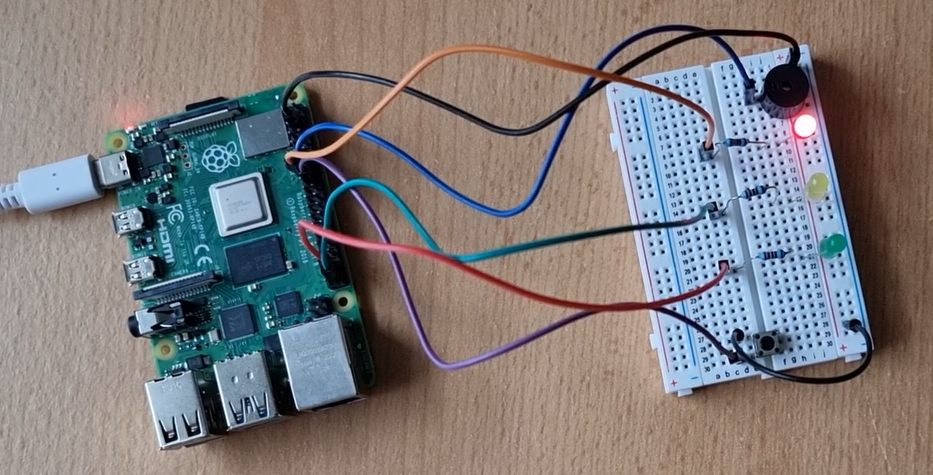
\includegraphics[width=0.8\textwidth]{images/Alarm_rot}
	\caption{Raspberry Pi mit angeschlossenem Alarm-Hardware-System (rot)}
	\label{fig:alarm_system_red}
\end{figure}

Im normalen Betriebszustand, wenn alles in Ordnung ist, leuchtet die grüne LED (siehe Abbildung \ref{fig:alarm_system}). Bei einer Fall-Detection, wenn ein Patient gestürzt ist, leuchtet die rote LED und der Buzzer gibt ein akustisches Signal aus. Der Taster kann verwendet werden, um den Buzzer stummzuschalten (siehe Abbildung \ref{fig:alarm_system_red}). Die gelbe LED kann für weitere Signalisierungen verwendet werden.
